\chapter{RESEARCH METHODOLOGY}
%This chapter of a thesis commences a brief statement and enumerating the main topics that are to be covered in it; namely; 
%(1) Research Design; 
%(2) Sources of Data (Locale of the Study and Population/Sampling); 
%(3) Instrumentation and Data Collection; and 
%(4) Tools for Data Analysis. Writing chapter 3 of a thesis requires the assistance of a statistician (in most cases). This is because it is in this chapter that the thesis writer is usually required to indicate what statistical tools he intends to use in data analysis. Here is the basic format of Chapter 3. 

% =========================================================
%\section{Research Design}
% =========================================================
%The appropriate research design should be specified and described (including requirement, modeling and detailed description of system/product/method development.
%\subsection{System/product/method Implementation}
%Describe the place where the study was conducted and the rationale behind its choice, the environment of the system (device specification, tools specification and language, which were used in the implementation)
%\subsection{Experiment Scenario}
%Describe the experiment scenario (including the objective, the procedure of the experiment and the variable which will be used in the experiment).

% =========================================================
%\section{Population/Sampling}
% =========================================================
%Describe the population of interest and the sampling of subjects used in the study.

% =========================================================
%\section{Instrumentation and Data Collection}
% =========================================================
%Describe the instrument, what it will measure, how to interpret. Discuss how the validity and the reliability will be established. Specify the level of reliability (probability). Give details of instruction given to assistants if persons other than the researcher gather data. State qualifications of informants if used in the study.

% =========================================================
%\section{Tools for Data Analysis}
% =========================================================
%Determine and justify the statistical treatment for each sub-problem, the scales of values used and the descriptive equivalent ratings, if any.
Desain Autonomous Trash Collector Robot memerlukan beberapa hardware diantaranya single board computer, embedded board, actuator, baterai dan sensor kamera.
Actuator yang digunakan dalam penelitian ini yaitu dinamo motor DC 12V yang berguna sebagai penggerak dengan tegangan arus yang searah dengan kumparan medan agar diubah menjadi gerak mekanik. Embedded board yang digunakan adalah driver motor L298N yang berfungsi untuk menjalankan actuator, mengatur arah dan kecepatan pada sebuah actuator. Single Board Computer (SCB)  yang berfungsi sebagai otak sehingga mengatur sistem yang ada dan komunikasi sistem dalam robot. Sensor kamera di sini menggunakan 1 buah sensor kamera (monocular camera), kamera di sini dibutuhkan sebagai sensor utama pada robot yang berfungsi sebagai alat bantu robot untuk melakukan tugasnya dan terintegrasi langsung pada SCB robot.

Behavior based robotic merupakan sistem kontrol berbasis pada level kompetensi dan koordinator tertentu. Maka dibutuhkan beberapa tahapan perancangan algoritma untuk diterapkan pada Autonomous Trash Collector Robot (ATCR). Tahapan menghindari halangan, mecari target, dan menuju target. Tahapan perilaku tersebut dilakukan pembelajaran dengan menggunakan algoritma Neuro Fuzzy Q-Learning (NFQL).
Robot dikendalikan secara langsung pada pengendali tingkat bawah (low level controller) berupa kontroler P yang berfungsi mengendalikan aktuator motor driver dan motor DC. Robot juga akan mengirimkan sinyal persepsi, melalui sensor kamera pada pengendali tingkat atas (High Level Controller). Kemudian sinyal tersebut menjadi masukan untuk mengaktifkan behavior koordinasi. Output behavior coordination mengaktifkan low level controller agar mengendalikan  robot. 



%OVERVIEW/RINGKASAN

\section{Model system dan Skenario} 
Robot akan dikendalikan secara langsung oleh low
level controller (berupa kontroler P) yang berfungsi
untuk mengendalikan pergerakan robot dengan beberapa motor DC yang ada. Robot juga akan
mengirim sinyal persepsi (melalui sensor – sensor
yang dimilikinya) pada high level controller.
Kemudian sinyal tersebut menjadi masukan stimulus
yang akan mengaktifkan behavior – behavior tertentu
(yang dikoordinasi oleh bagian behavior coordination).
Output dari behavior coordination diberikan pada low level controller untuk pengendalian robot.  Diagram Blok Keseluruhan sistem robot seperti pada Gambar \ref{fig:NFQL_BBR_AMR} berikut ini.
 
 \begin{figure}[H]
 	\centering
 	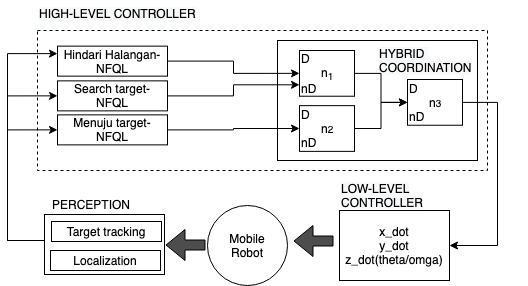
\includegraphics[width=5.5in]{figure/NFQL-BBR-AMR}
 	\caption{Behavior Based Kontrol pada Autonomous Trash Collector Robot}
 	\label{fig:NFQL_BBR_AMR}
 \end{figure}
 


% =========================================================
%\subsection{Autonomous Mobile Robot Overview}
% =========================================================
%Perancangan yang akan dibangun adalah non-platform mobile robot, oleh karena itu diperlukan penempatan sensor yang tepat agar robot dapat melaksanakan tugasnya sesuai apa yang diinginkan. Di bawah ini ditunjukan peletakan komponen hardware pada robot:

%skematik hardware ATCS 
%\subsection{Design}


%Gambar 3. 2 Ilustrasi perancangan robot


%hardware 
%mekanik robot
%spesifikasi mekanik robot

%software

%Gambar 3.2 merupakan ilustrasi tentang perancangan robot, berikut ini adalah penjelasan tentang perancangan robot yang tertera pada gambar 3.1 :
%1. Pada lapisan 1 terdapat 2 actuator sebagai penggerak, 1 driver motor L298N dan 1 baterai berkapasitas 1550mAh.
%2. Pada lapisan 2 terdapat Single Board Computer (SCB) yaitu Raspberry pi 3B+ sebagai otak robot dan power distribution board yang berfungsi untuk sumber tegangan untuk SCB dan actuator.
%3. Pada lapisan 3 terdapat USB Camera yang sudah tersambung dengan SCB melalui port USB.
%Gambar 3. 3 Bentuk mobile robot yang dilengkapi dengan sensor kamera


%\subsection{Actuators}

%\subsection{Sensing}
%kebutuhan hardware (perangkat keras) dan software (perangkat lunak) untuk perancangan sistem mobile robot secara keseluruhan. Berikut adalah uraiannya:
%Tabel 3. 1 Komponen Hardware dan Software

	
% =========================================================

% =========================================================

% Software Architecture
% =========================================================
%\section{Software Architecture}
% =========================================================



%==========================================================


%Berisi asumsi system yang diamati/diobservasi dan scenario proses system beserta asumsi dan batasan system. Perlu dijelaskan sub system-sub system pembangun model system tersebut. Dilengkapi dengan gambar system dan sub system yang diamat. 
%Berisi minimal 1 halaman.

\section{Skenario Simulasi }
%Berisi penjelasan scenario simulasi real atau simulasi menggunakan alat bantu software. 
%Berisi minimal 1 halaman.
\subsection{Target Tracking}
% =========================================================
%algoritma image processing
%CNN
%5.3.1.2 Deep Learning for Autonomous Driving
Agar mendapatkan hasil prediksi tindakan terbaik, robot pada kondisi tertentu di lingkungan, perlu mengklasifikasikan informasi kondisi yaitu gambar kamera selaras dengan aksi. Banyak algoritma klasifikasi yang berbeda tetapi   Convolutional Neural Networks
(CNN) model digunakan untuk masalah penelitian ini.
Motivasi menggunakan CNN di atas teknik klasifikasi atau jaringan saraf lainnya adalah bahwa CNN memanfaatkan pola dan informasi struktural secara efisien dalam sebuah gambar. Adapun misalnya, di RNN, ketergantungan keluaran pada semua nilai sebelumnya menghasilkan gambar yang sangat buruk. Selain itu, kebutuhan memori yang lebih sedikit dan parameter yang lebih sedikit. Saat menargetkan model untuk robot dengan daya komputasi rendah, CNN baik untuk digunakan.

%\subsection{Image Segmentation}

%\subsection{Target Normalization Position}

%\subsection{Velocity Estimation}
Proses pertama yang dilakukan setelah menangkap citra adalah melakukan preprocessing.
Hasil dari preprocessing adalah citra dalam bentuk threshold (citra hitam dan putih). Citra threshold akan diproses lagi di dalam CNN untuk ektraksi fitur dan diklasifikasikan. Pada metode CNN akan berusaha membuat klasifikasi citra semirip mungkin dengan dataset yang dimiliki. Perancangan perangkat lunak dari preprocessing dan klasifikasi citra pada CNN menggunakan perangkat lunak PyCharm dengan bahasa pemrograman python dan library OpenCV dan tensorflow.
Setelah citra diklasifikasi akan mengirimkan sinyal dalam bentuk data yang akan diterima oleh High level controller. Data
yang masuk menjadi pergerakan motor. 

% =========================================================
\subsection{Localization System}

%algoritma hidari halangan and searching

%algoritma menuju target


Perancangan behavior untuk pencarian sampah:

\begin{enumerate}
	\item Menghindar halangan dan Mencari target
	
 Tujuannya adalah menghindari setiap halangan yang dideteksi oleh senso kamera. Behavior ini belajar menggunakan Neuro-Fuzzy Q-Learning (FQL). 
Dengan sensor kamera, robot berupaya mencari posisi target. Selama tidak ada halangan, tidak tabrakan, behavior ini akan diaktifkan penuh. Jika target tidak terdeteksi, aktivasi bernilai 1, sehingga robot berusaha mencari target.

\item Menuju target

Behavior ini memiliki tingkat aktivasi paling rendah. Dia akan aktif penuh jika behavior-behavior sebelumnya tidak aktif. Setelah target didapatkan oleh behavior “mencari target”,dengan behavior ini, robot akan menuju target.

\end{enumerate}


\section{Desain Lingkungan}
Lingkungan memiliki objek dan rintangan yang diletakan secara acak.  Sementara sensor kamera dalam mengidentifikasi objek dan rintangan yang ditemui di jalurnya. Serta membantu robot untuk menavigasi dalam arena berukuran 2m x 2m.





%================================================================

\section{Skenario Pengambilan data}
%Berisi scenario pengambilan data dari hasil simulasi real / alat bantu software. Definisikan parameter yang diobservasi dan cara mendapatkan parameter-parameter tersebut. 

%Berisi minimal 1 halaman.


Untuk memastikan tingkat akurasi tertentu, pada thesis ini akan menggunakan “Confusion Matrix” untuk membandingkan klasifikasi prediksi dengan klasifikasi sebenarnya, teknik yang biasa digunakan ketika membandingkan pengklasifikasi pembelajaran seperti jaringan saraf, tidak hanya mendapatkan akurasi untuk dihitung, tetapi juga sensitivitas dan spesifisitas solusi. 

Sensitivitas solusi adalah kemampuannya untuk menghindari mengabaikan hasil positif, sedangkan spesifisitas adalah kemampuan solusi untuk mengklasifikasikan negatif yang benar dengan benar. Kedua ukuran statistik berguna saat mengukur kemampuan detektor objek untuk tujuan mengemudi otonom – nilai sensitivitas rendah dapat mencegah sistem deteksi objek mengidentifikasi rintangan pada waktunya untuk menghindari tabrakan. Oleh karena itu, solusi harus memiliki sensitivitas yang sangat tinggi untuk memastikan tingkat keandalan praktis.

Selain itu, solusi harus memiliki kekhususan yang signifikan sehingga tidak salah mengklasifikasikan objek dari latar belakang. Hal ini terutama berlaku dalam hal mendeteksi obyek dan rintangan,  mungkin memiliki efek yang tidak diinginkan saat diproses oleh sistem navigasi (seperti mengemudi dengan kecepatan sangat tinggi jika salah mendeteksi obyek).
Selain itu, solusi harus cukup cepat untuk dilakukan secara real time. 
%Sementara definisi "waktu nyata" sangat berbeda antara arsitektur yang diusulkan (Ren et al. 2017, Redmon et al. 2018), pergerakan robot EyeBot yang relatif lambat dan kemampuan perangkat kerasnya yang terbatas memungkinkan waktu inferensi menjadi lebih tinggi. 



%Parameter pengujian yang akan diteliti adalah sebagai berikut:
%	\item Learning rate α
%	A diverse set of values were tested. The final learning rate was set to α = 0.1, which demonstrated a fast and stable learning process.
	
%	\item Discount factor γ.
%	The discount factor was set to γ = 0.9. Since the learning of a robot behavior is a continuous task without a final state, a discount factor smaller than 1 was required. In the case of using γ = 1.0, the Q function values would increase or decrease, depending on the state/action zone, until they reach −∞ or ∞. This value was chosen experimentally without exploring many values.
	
%	\item Exploration probability ?.
%	The learning was performed with a ?−greedy policy. The exploration probability was ? = 0.3. A smaller exploration probability increased the time required to converge, and a higher prob- ability caused the robot to act too randomly. The value was also set experimentally.
%	Database
	
%	\item Database Density Parameter t. The density parameter was set to t = 0.5. However, this parameter does not provide intuitive information about the number of learning samples. It indicates the minimum dis- tance between two learning samples. This distance is calculated ac- cording to the vectors (s, a, r) of each sample, which, in this case was a four-dimensional vector since the state has two dimensions. In prac- tice, the number of learning samples resulted in being less than 30, although it depended on the state/action space exploration. Several parameters were tested, concluding that with a larger value (less sam- ples) the convergence was not always achieved due to the interference problem. Similar results were obtained for both DOFs.

%Ren, S., He, K., Girshick, R. and Sun, J. (2017). Faster R-CNN: Towards Real-Time Object Detection with Region Proposal Networks. IEEE Transactions on Pattern Analysis and Machine Intelligence, [online] 39(6), pp.1137-1149. Available at: https://ieeexplore.ieee.org/document/7485869/

%\subsection{Deteksi Obyek}
%diagram alir deteksi obyek
\section{Skenario Analisis}
%Berisi scenario analisis hasil pengambilan data. 
%Berisi minimal 1 halaman.

Untuk menguji algoritma kontrol pada ATCS, dilakukan beberapa tahapan:

\begin{enumerate}
	\item Pembuatan model 3D Robot. Model 3D diperlukan untuk keperluan simulasi algoritma kontrol robot menggunakan program 3D. Simulator robot 3D yang dapat digunakan untuk mendesain model 3D robot, membuat script pemrograman dan melakukan simulasi robot seperti kondisi real robot.

\item Simulasi Algoritma kontrol pada model robot. Hasil desain algoritma diujicobakan pada simulator robot sebelum diujicobakan pada robot sebenarnya. Simulator ini dibuat mengunakan software simulator dengan pemrograman algoritma kontrol.

\item Implementasi Algoritma pada robot sebenarnya. Setelah simulasi algoritma kontrol pada simulator robot berhasil, algoritma kontrol ditanam pada robot sebenarnya.
\item Pengujian Sistem robot pada medan sebenarnya. Analisa untuk akurasi robot dilakukan dengan membandingkan titik uji dengan titik yang dihasilkan oleh gerakan. Dari selisih kedua titik tersebut akan didapatkan akurasi dari robot.  Analisa error pergerakan dilakukan dengan membandingkan bentuk data target dan hasil proses. Dari selisih waktu dan jarak yang dihasilkan akan didapatkan error pergerakan.
\end{enumerate}